\chapter*{Dodatak: Prikaz aktivnosti grupe}
		\addcontentsline{toc}{chapter}{Dodatak: Prikaz aktivnosti grupe}
		
		\section*{Dnevnik sastajanja}
		
	%	\textbf{\textit{Kontinuirano osvježavanje}}\\
		
	%	 \textit{U ovom dijelu potrebno je redovito osvježavati dnevnik sastajanja prema predlošku.}
		
		\begin{packed_enum}
			\item  sastanak
			
			\item[] \begin{packed_item}
				\item Datum: 17. listopada 2022.
				\item Prisustvovali: P. Hajduk., M. Čengić, N. Capan, J. Jakovac
				\item Teme sastanka:
				\begin{packed_item}
					\item  Predstavljanje nove teme za prijedlog
					\item  Rasprava o novoj temi za prijedlog
					\item  Rasprava o mogućoj podjeli rada
					\item  Teambuilding
				\end{packed_item}
			\end{packed_item}
			
			\item  sastanak
			\item[] \begin{packed_item}
				\item Datum: 14. studenoga 2022.
				\item Prisustvovali: P. Hajduk., M. Čengić, N. Capan, J. Jakovac, M. Balog, I. Baričević, L. Čunović
				\item Teme sastanka:
				\begin{packed_item}
					\item  Rasprava o implementacijskim detaljima
					\item  Rasprava o daljnjim koracima
				\end{packed_item}
			\end{packed_item}
			
			\item  sastanak
			\item[] \begin{packed_item}
				\item Datum: 04. prosinca 2022.
				\item Prisustvovali: P. Hajduk., M. Čengić, N. Capan, J. Jakovac, M. Balog, I. Baričević
				\item Teme sastanka:
				\begin{packed_item}
					\item  Rekapitulacija detalja napravljenog
					\item  Rasprava o bazičnim stavkama funkcionalnosti aplikacije
				\end{packed_item}
			\end{packed_item}
			
		\end{packed_enum}
		
		\eject
		\section*{Tablica aktivnosti}
		
		%	\textbf{\textit{Kontinuirano osvježavanje}}\\
			
		%	 \textit{Napomena: Doprinose u aktivnostima treba navesti u satima po članovima grupe po aktivnosti.}

			\begin{longtblr}[
					label=none,
				]{
					vlines,hlines,
					width = \textwidth,
					colspec={X[7, l]X[1, c]X[1, c]X[1, c]X[1, c]X[1, c]X[1, c]X[1, c]}, 
					vline{1} = {1}{text=\clap{}},
					hline{1} = {1}{text=\clap{}},
					rowhead = 1,
				} 
				\multicolumn{1}{c|}{} & 
				\multicolumn{1}{c|}{\rotatebox{90}{\textbf{Petar Hajduk}}} & \multicolumn{1}{c|}{\rotatebox{90}{\textbf{Jakov Jakovac}}} &	\multicolumn{1}{c|}{\rotatebox{90}{\textbf{Matej Balog}}} & \multicolumn{1}{c|}{\rotatebox{90}{\textbf{Ivor Baričević}}} &	\multicolumn{1}{c|}{\rotatebox{90}{\textbf{Marko Čengić}}} & \multicolumn{1}{c|}{\rotatebox{90}{\textbf{Nikola Capan}}} &	\multicolumn{1}{c|}{\rotatebox{90}{\textbf{Lovro Čunović}}} \\  
				Upravljanje projektom 		& 0 & 18 & 0 & 0 & 2 & 0 & 0 \\ 
				Opis projektnog zadatka 	& 0 & 10 & 0 & 0 & 0 & 0 & 2 \\ 
				
				Funkcionalni zahtjevi       & 0 & 1 & 0 & 0 & 2 & 0 & 0 \\ 
				Opis pojedinih obrazaca 	& 0 & 3 & 0 & 0 & 8 & 0 & 0 \\ 
				Dijagram obrazaca 			& 0 & 0 & 0 & 0 & 4 & 0 & 0 \\ 
				Sekvencijski dijagrami 		& 0 & 0 & 0 & 0 & 4 & 0 & 0 \\ 
				Opis ostalih zahtjeva 		& 0 & 0 & 0 & 0 & 1 & 0 & 0 \\ 

				Arhitektura i dizajn sustava	 & 0 & 3 & 0 & 0 & 0 & 0 & 2 \\ 
				Baza podataka				& 2 & 2 & 0 & 0 & 0 & 7 & 0 \\ 
				Dijagram razreda 			& 0 & 0 & 0 & 0 & 0 & 8 & 0 \\ 
				Dijagram stanja				& 0 & 0 & 0 & 0 & 2 & 0 & 0 \\ 
				Dijagram aktivnosti 		& 0 & 0 & 0 & 0 & 2 & 0 & 0 \\ 
				Dijagram komponenti			& 0 & 0 & 0 & 0 & 2 & 0 & 0 \\ 
				Korištene tehnologije i alati 		& 0 & 2 & 0 & 0 & 0 & 0 & 0 \\ 
				Ispitivanje programskog rješenja 	& 3 & 2 & 0 & 0 & 0 & 2 & 0 \\ 
				Dijagram razmještaja			& 0 & 0 & 0 & 0 & 2 & 2 & 0 \\ 
				Upute za puštanje u pogon 		& 0 & 2 & 0 & 0 & 0 & 0 & 0 \\  
				Dnevnik sastajanja 			& 0 & 1 & 0 & 0 & 0 & 0 & 0 \\ 
				Zaključak i budući rad 		& 0 & 0 & 0 & 0 & 1 & 0 & 0 \\  
				Popis literature 			& 0 & 0 & 0 & 0 & 1 & 0 & 0 \\ \hline  
				 
				{Dizajn aplikacije} 				& 0 & 13 & 1 & 1 & 0 & 0 & 0 \\ 
				{Rad na responzivnosti aplikacije} 				& 0 & 0 & 0 & 0 & 0 & 0 & 0 \\ 
				{Implementacija Login/Logout} 				& 0 & 7 & 0 & 0 & 0 & 0 & 0 \\ 
				{Implementacija Razina ovlasti} 				& 0 & 0 & 0 & 0 & 0 & 0 & 0 \\ 
				{Izrada headera} 				& 0 & 8 & 0 & 2 & 0 & 0 & 0 \\  
				{Izrada naslovnice} 				& 0 & 1 & 0 & 0 & 0 & 0 & 0 \\  
				{Izrada users stranice} 		 			& 0 & 1 & 4 & 3 & 0 & 0 & 0 \\  
				{Izrada user forme} 							& 0 & 4 & 0 & 2 & 0 & 0 & 0 \\ 
				{Izrada delete forme} 							& 0 & 0 & 0 & 1 & 0 & 0 & 0 \\ 
				{Izrada projects stranice} 							& 0 & 3 & 5 & 0 & 0 & 0 & 0 \\ 
				{Izrada project forme} 							& 0 & 0 & 4 & 0 & 0 & 0 & 0 \\ 
				{Izrada companies stranice} 							& 0 & 2 & 4 & 0 & 0 & 0 & 0 \\ 
				{Izrada company forme} 							& 0 & 0 & 3 & 0 & 0 & 0 & 0 \\ 
				{Izrada collaborations komponente} 							& 0 & 4 & 2 & 3 & 0 & 0 & 0 \\ 
				{Izrada spring backenda} 							& 17 & 1 & 0 & 2 & 0 & 11 & 0 \\  
				{Deploy aplikacije} 							& 0 & 7 & 0 & 0 & 0 & 0 & 0 \\
			\end{longtblr}
					
					
		\eject
		
		\section*{Dijagrami pregleda promjena}
		
		% \textbf{\textit{dio 2. revizije}}\\
		
		% \textit{Prenijeti dijagram pregleda promjena nad datotekama projekta. Potrebno je na kraju projekta generirane grafove s gitlaba prenijeti u ovo poglavlje dokumentacije. Dijagrami za vlastiti projekt se mogu preuzeti s gitlab.com stranice, u izborniku Repository, pritiskom na stavku Contributors.}
		
	
		\begin{figure}[H]
			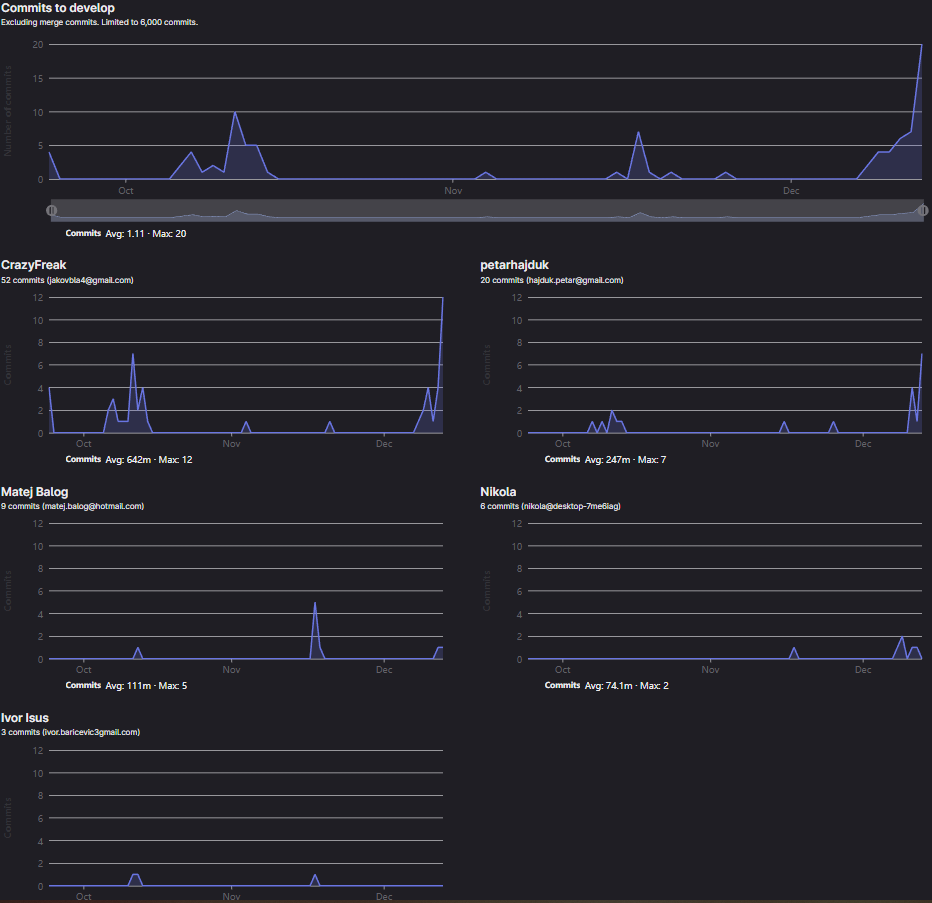
\includegraphics[width=\textwidth]{slike/commits-develop.png} %veličina u odnosu na širinu linije
			\caption{Prikaz aktivnosti na repozitoriju za granu develop}
			\label{fig:CommitsDevelop} %label mora biti drugaciji za svaku sliku
		\end{figure}
  
		\begin{figure}[H]
			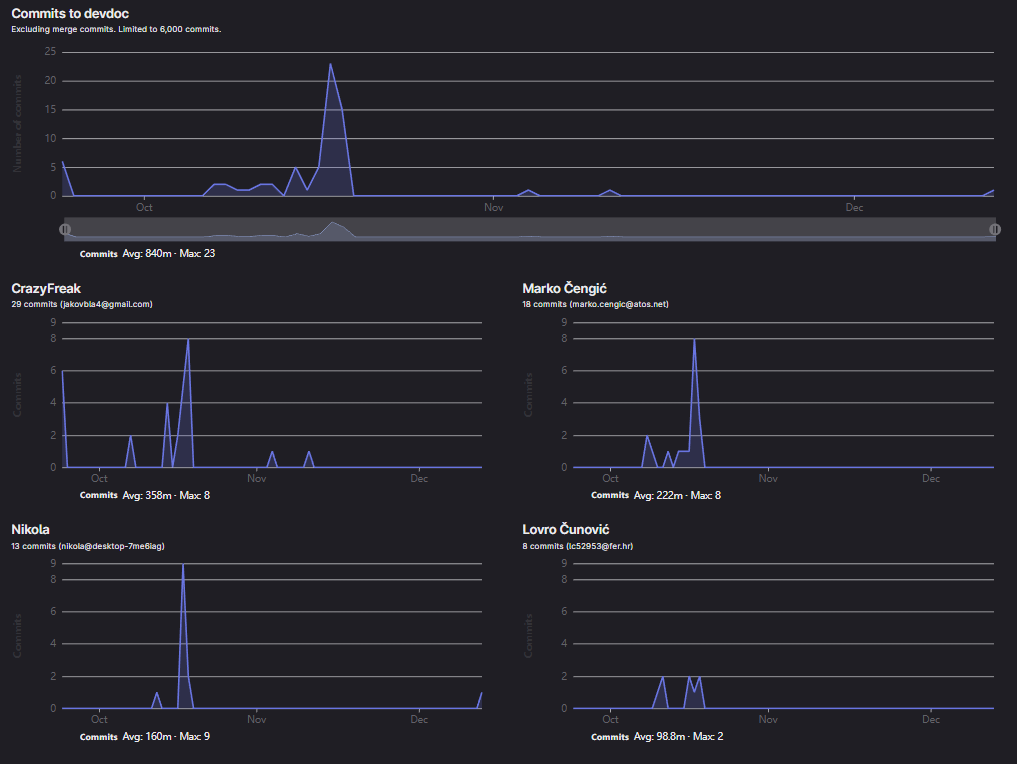
\includegraphics[width=\textwidth]{slike/commits-devdoc.png} %veličina u odnosu na širinu linije
			\caption{Prikaz aktivnosti na repozitoriju za granu devdoc}
			\label{fig:CommitsDevdoc} %label mora biti drugaciji za svaku sliku
		\end{figure}